%中間審査概要テンプレート ver. 3.0

\documentclass[uplatex,twocolumn,dvipdfmx]{jsarticle}
\usepackage[top=22mm,bottom=22mm,left=22mm,right=22mm]{geometry}
\setlength{\columnsep}{10mm}
\usepackage[T1]{fontenc}
\usepackage{txfonts}
\usepackage[expert,deluxe]{otf}
\usepackage[dvipdfmx,hiresbb]{graphicx}
\usepackage[dvipdfmx]{hyperref}
\usepackage{pxjahyper}
\usepackage{secdot}





%タイトルと学生番号,名前だけ編集すること
\title{\vspace{-5mm}\fontsize{14pt}{0pt}\selectfont GitHubにおける人的資源マネジメント}
\author{\normalsize プロジェクトマネジメントコース 矢吹研究室 1342081 氏名 辻岡 大知}
\date{}
\pagestyle{empty}
\begin{document}
\fontsize{10.5pt}{\baselineskip}\selectfont
\maketitle





%以下が本文
\section{背景}

ソフトウェア開発では,GitHubを用いることが多い.GitHubとはコンピュータ上で作成,編集されるファイルの変更履歴を管理するためのバージョン管理システムである.1000万人以上ものユーザがGitHubを活用しコードなどを共有しプロジェクトを行っている.


システムエンジニアはコミュニケーション能力が必要とされる仕事である.私はGitHubに公開されているプロジェクトを調べているうち,活発に活動しているユーザはGoogle+やTwitterで交友関係が広い場合が多いことに気が付いた.そこで私はGitHubを用い,活発に活動するシステムエンジニアはコミュニティが広いのではないかという仮説を立て,その仮説を検証するため本研究を行った.


\section{目的}

ソフトウェア開発で活発に活動しているユーザはコミュニティが広いのではないかという仮説を検証する.

\section{手法}

活発に活動しているシステムエンジニアのユーザ情報を集めるためGHTorrentを使用した.GHTorrentとはGitHubのあらゆる情報が格納されているダンプファイルのことである.

活発に活動しているシステムエンジニアのコミュニティを調べるため,GitHubの機能の一つであるcontributionとGoogle+を使用した.contributionとはユーザがどの程度GitHub上で活動しているのかを定量的に知ることのできる値である.

集めたユーザのコミュニティ関係を調べるためGoogle+を使用した.Google+とはGoogleが運営するSNSのことである.

以下のような手順で研究を進めた.

\begin{enumerate}
 \item GHTorrentから2万件のユーザ情報をランダムサンプリングで抽出した.
 \item 1で抽出したユーザのメールアドレスを,GitHubAPIを用いて取得した.
 \item 取得したメールアドレスを用いGoogle+におけるフォロワー数を調べた.
 \item ユーザのcontribution数とGoogle+におけるフォロワー数の相関関係を調べた.
\end{enumerate}

\section{結果}

%図の挿入
\begin{figure}[htb]
\centering
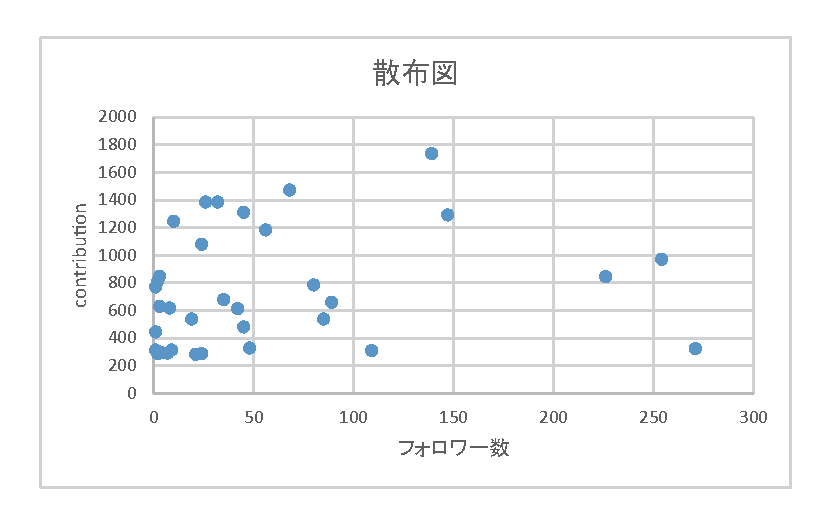
\includegraphics[width=7cm]{figure.pdf}
\caption{contribution数とフォロワー数の相関}\label{サンプル図}
\end{figure}

本研究の結果が図1の散布図である.この散布図により,GitHubにおけるcontribution数とGoogle+におけるフォロワー数に相関関係はないということが分かった.

\section{考察}

本研究を通して,活発に活動しているユーザはGoogle+におけるコミュニティが必ずしも広いわけではないことが分かった.今回研究を行うためGoogle+というSNSを用いたが,現在流行しているFacebookやTwitterなどのSNSを用いることにより,今回とは違った結果が得られるのではないかと考えた.

\section{結論}

本研究を通して明らかとなった相関関係などはなかった.しかし研究を進めるための過程でGHTorrent及びGoogleAPIを使用することができるようになった.今後の課題として研究を行う段階で最も流行しているSNSなどでデータを取得し,統計を取っていく必要がある.





\end{document}
